\documentclass{beamer}
\usepackage[utf8]{inputenc}
\usepackage[graphicx]

\author[Sowmya Vajjala]{Instructor: Sowmya Vajjala}


\title[LING 120]{Language and Computers}
\subtitle{Semester: FALL '17}

\date{20 October 2017}

\institute{Iowa State University, USA}

%%%%%%%%%%%%%%%%%%%%%%%%%%%

\begin{document}

\begin{frame}\titlepage
\end{frame}

\begin{frame}
\frametitle{Outline}
\begin{enumerate}
\item Recap of last class
\item how does learning happen?
\item reminder: Assignment 4 is due tomorrow!!
\end{enumerate}
\end{frame}

\begin{frame}
\frametitle{What is Text classification?}
\begin{itemize}
\item If we have some amount of example corpus which has some kind of known categorization, text classification is the method which uses these examples to learn to categorize new texts. \pause
\item Applications: spam filtering, email categorization, reachout.com forum posting severity detection, language identification, checking whether a web page is suitable for children or not etc.
\end{itemize}
\end{frame}

\begin{frame}
\frametitle{Steps in Text classification?}
\begin{itemize}
\item We need a collection of example texts with known categories (Training data)
\item We need to extract "features" we want the machine to learn from these (feature extraction)
\item We should take these extracted features and give them to a "learning algorithm" (training/learning phase)
\item Evaluate if the "learned" classifier is doing well by "testing" it with a few more examples with known categories (test data, evaluation)
\item If you are happy, start using in some real-world application!!
\end{itemize}
\end{frame}

\begin{frame}
\frametitle{Recap questions}
\framesubtitle{... with Random questioning}
Let us take "spam classification" as our example problem.
\begin{itemize}
\item Where can we get the training data for this? \pause
\item What features are meaningful? \pause
\item How do we get these features? \pause
\item What happens after feature extraction? \pause
\item What according to you is a good way to evaluate the classification?
\end{itemize}
\end{frame}

\begin{frame}
\frametitle{The attendance question from last class}
\begin{itemize}
\item Problem: Understanding how to figure out which of those descriptions are by a human, or a machine, or identify unclear cases.
\item Logic: Looking at the example descriptions, we should build a notion of whether those adjectives have similar meanings or opposite meanings, and use that knowledge to solve for unknown cases.
\item This is an example of text classification, except that we are doing it manually, and with a small set of examples. 
\item Full description: \url{http://nacloweb.org/resources/problems/2015/N2015-G.pdf}
\item Solution description: \url{http://nacloweb.org/resources/problems/2015/N2015-GS.pdf}
\end{itemize}
\end{frame}

\begin{frame}
\frametitle{Steps in Text classification?}
\begin{itemize}
\item \textbf{We need a collection of example texts with known categories (Training data)}
\item We need to extract "features" we want the machine to learn from these (feature extraction)
\item We should take these extracted features and give them to a "learning algorithm" (training/learning phase)
\item Evaluate if the "learned" classifier is doing well by "testing" it with a few more examples with known categories (test data, evaluation)
\item If you are happy, start using in some real-world application!!
\end{itemize}
\end{frame}

\begin{frame}
\frametitle{Let us say this is my "training data"}
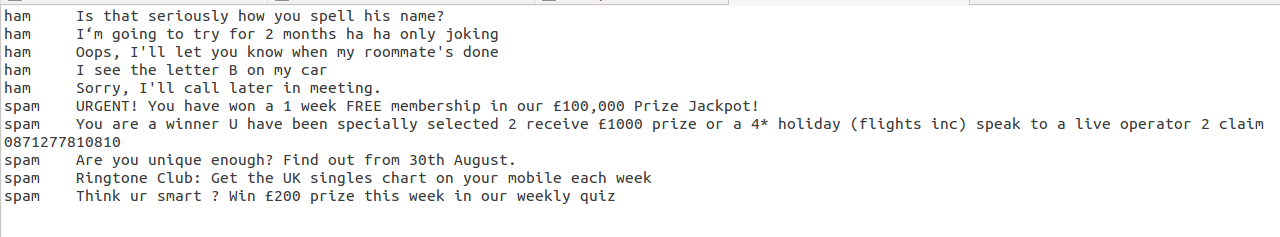
\includegraphics[width=0.9\textwidth]{ham-spam-example.png} \\
Note: In real life, training data is much larger. This is just for demonstration purposes.
\\ \pause If this is what I have, what is the next thing I should do? 
\end{frame}

\begin{frame}
\frametitle{Features}
\begin{itemize}
\item We need a collection of example texts with known categories (Training data)
\item \textbf{We need to extract "features" we want the machine to learn from these (feature extraction)}
\end{itemize}
What can we consider as features?
(Remember: our goal is to teach the computer to identify the language of spam emails versus ham emails)
\end{frame}

\begin{frame}
\frametitle{Features}
\begin{itemize}
\item Let us start with a simple (easy) idea of features - let us take all words as features.
\item Intuition: If a word occurs more frequently in Spam emails in the training data, perhaps its presence is indicative of spam in real-world emails.
\item So, in my training data, are there really such words???
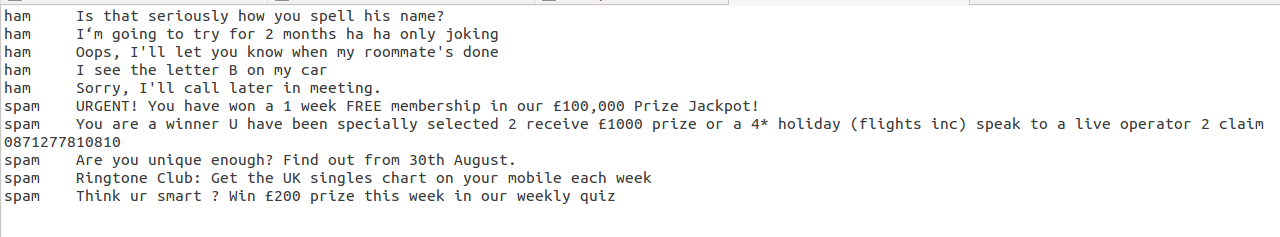
\includegraphics[width=0.9\textwidth]{ham-spam-example.png} \pause
\item How do I combine those 1000 pounds, 100K pounds, 200 pounds etc - to represent one feature? 
\end{itemize}
\end{frame}

\begin{frame}
\frametitle{Next step: Building up some evidence of word occurrences}
How?: by writing a computer program that counts word frequencies in Spam and Ham emails of training data.
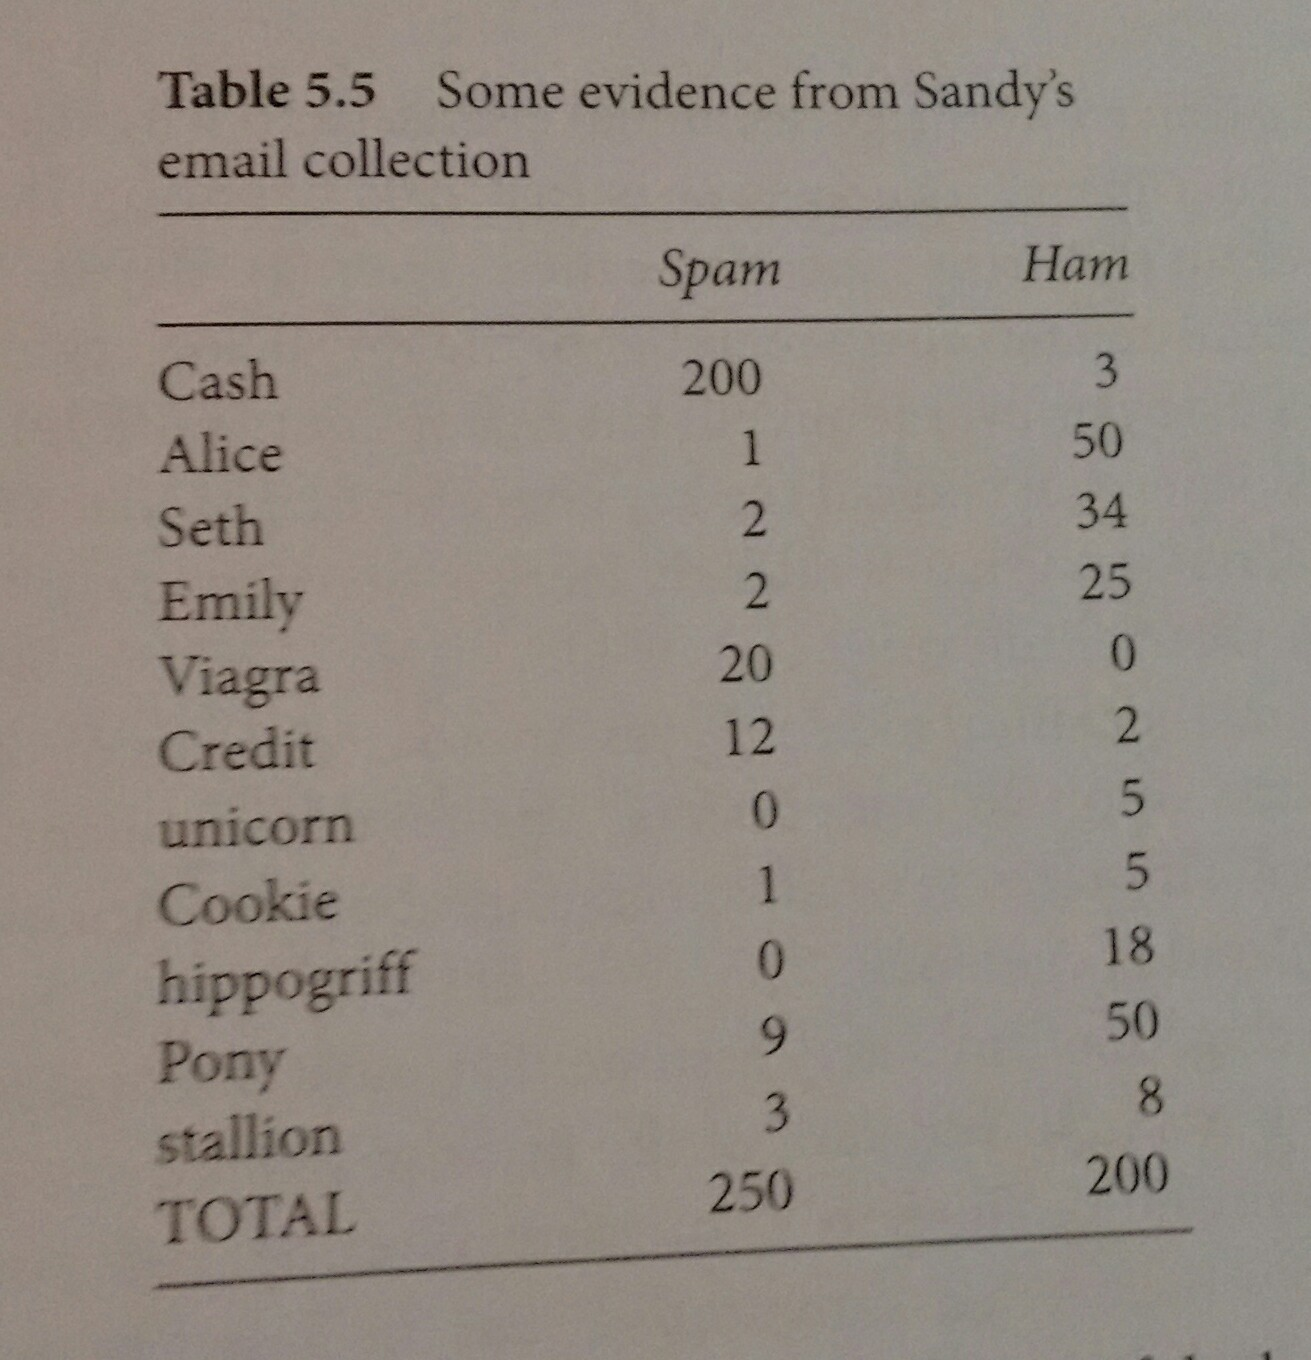
\includegraphics[width=0.5\textwidth]{spam-frequencies.jpg}
\\ Note: This is from textbook, not for the example data I showed. 
\end{frame}

\begin{frame}
\frametitle{Steps in Text classification?}
\begin{itemize}
\item We need a collection of example texts with known categories (Training data)
\item We need to extract "features" we want the machine to learn from these (feature extraction)
\item \textbf{We should take these extracted features and give them to a "learning algorithm" (training/learning phase)}
\end{itemize}
\end{frame}

\begin{frame}
\frametitle{So, how does "learning" happen?}
by observing stuff like:
\begin{itemize}
\item Cash appeared 203 times in total in the training data, of which 200 times was in Spam. What does this mean? \pause
\item Alice appeared 51 times in total, and 50 times in Ham. What is the probability that an sms is "Spam" if it has a single word "Alice"? \pause
\item Cookie appeared only 6 times in the entire corpus (total words: 450), and of which, it appeared 5 times. What does that mean? Is it a good feature? Does it indicate strong evidence? \pause
\item If Cash and Alice appeared in the message (not like a bigram, but just two separate words) - what inference can we draw? \pause
\item If credit and Alice appeared in the message, is it likely that this is spam, or not? 
\end{itemize}
\end{frame}

\begin{frame}
\frametitle{Once the computer calculates all these possibilities ...}
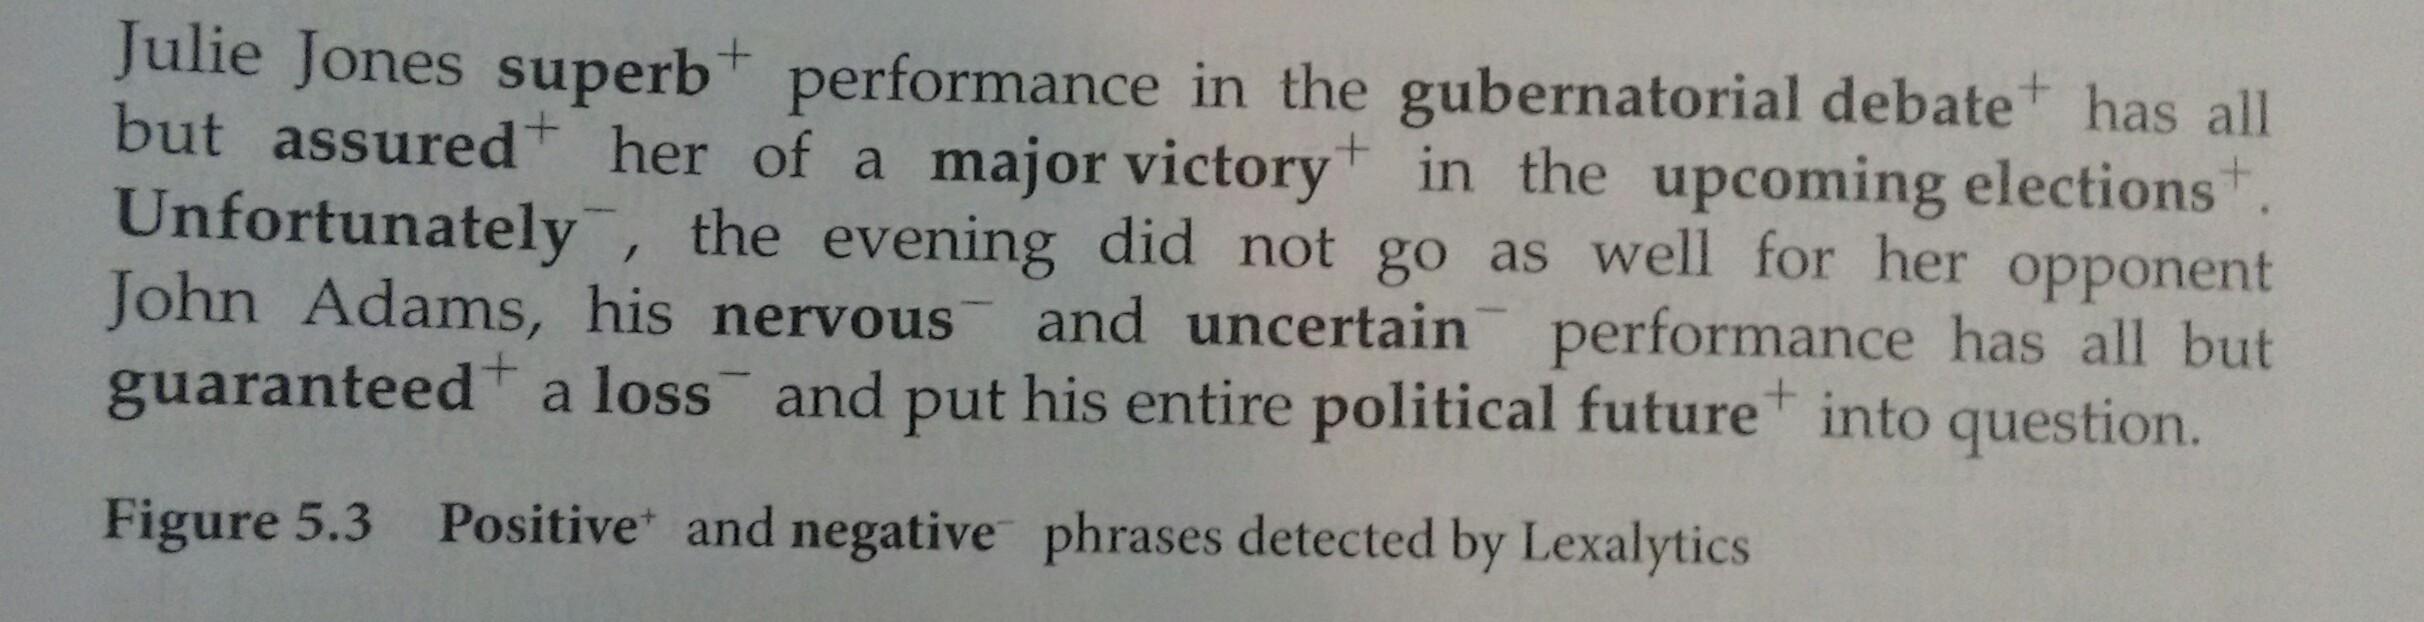
\includegraphics[width=0.9\textwidth]{classification-example.jpg} 
\end{frame}

\begin{frame}
\frametitle{How do we combine these multiple sources of information?}
Different learning algorithms do this differently. I will give an overview of some of these next week.
\end{frame}

\begin{frame}
\frametitle{Next week}
\begin{itemize}
\item How do we evaluate whether a learning algorithm is working? (Monday)
\item Different algorithms for learning - an introduction (Wednesday)
\item Conclusion of text classification and introduction to next topic (Dialog System)
\item ToDo: READ CHAPTER 5!
\item ToDo: Submit Assignment 4!
\end{itemize}
\end{frame}

\begin{frame}
\frametitle{Attendance Question}
In the five steps in text classification I mentioned earlier today, what do you think is the most difficult step for doing spam classification? Why?
\end{frame}


\end{document}
